\section{Empirical Evaluation}


\begin{figure*}[h]
\centering
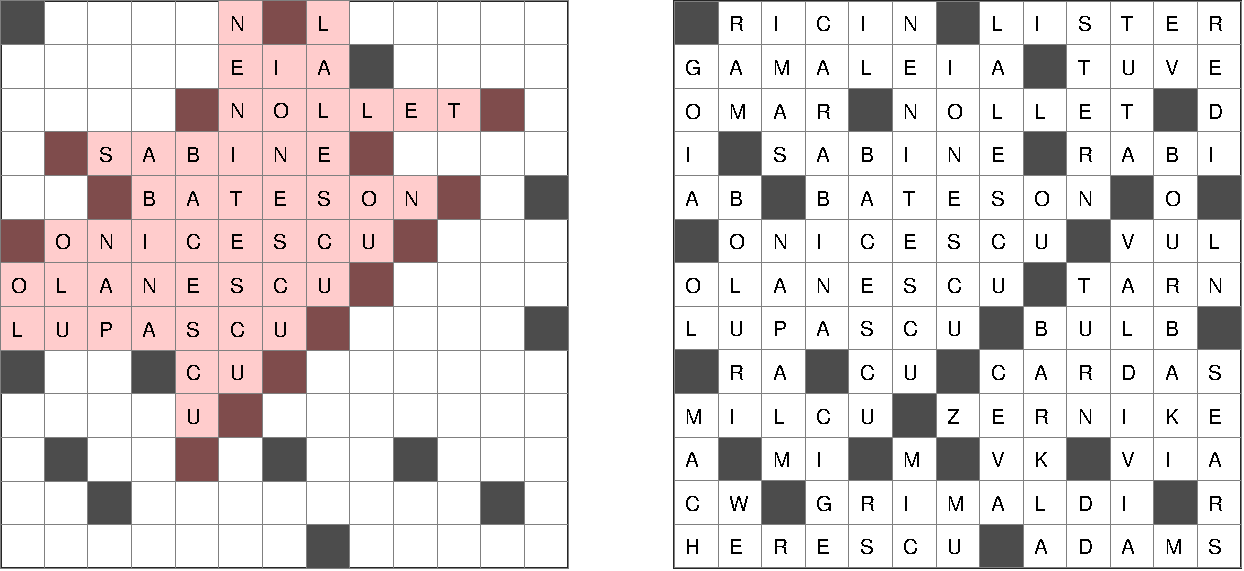
\includegraphics[width=0.6\textwidth]{_empiricalSupport/y-2013/results/_runWombat/mrmeGrids_y2013-60x932-14400x352-14113466-paper.pdf}

\vspace{0.25cm}

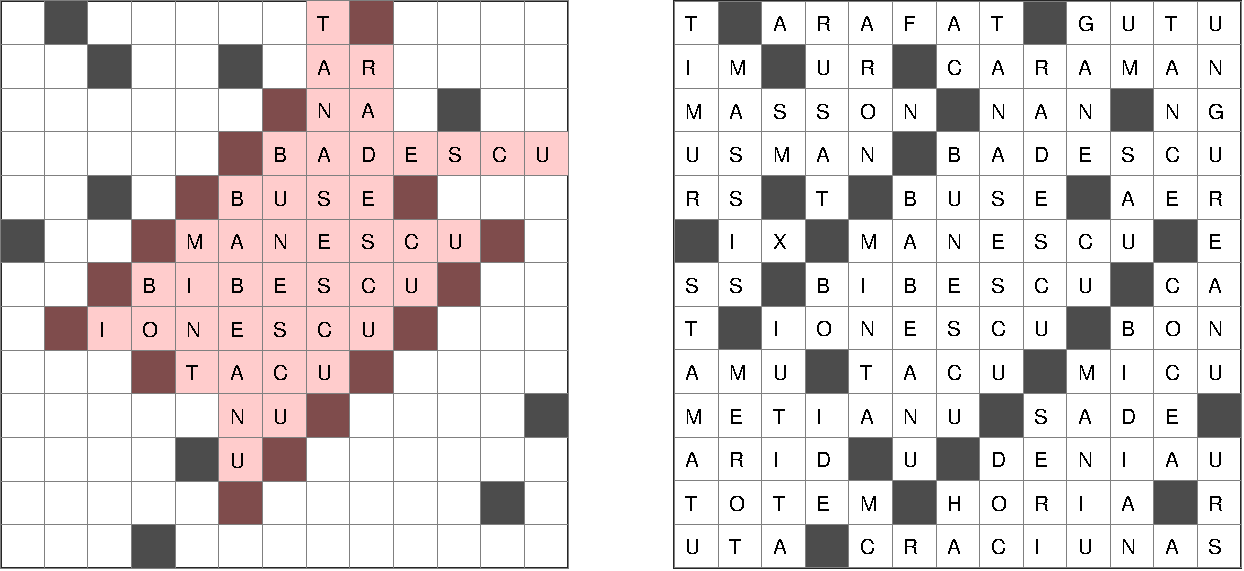
\includegraphics[width=0.6\textwidth]{_empiricalSupport/y-2021/results/_runWombat/mrmeGrids_feb3-60x38035-14400x224-13741779-paper.pdf}

\vspace{0.25cm}

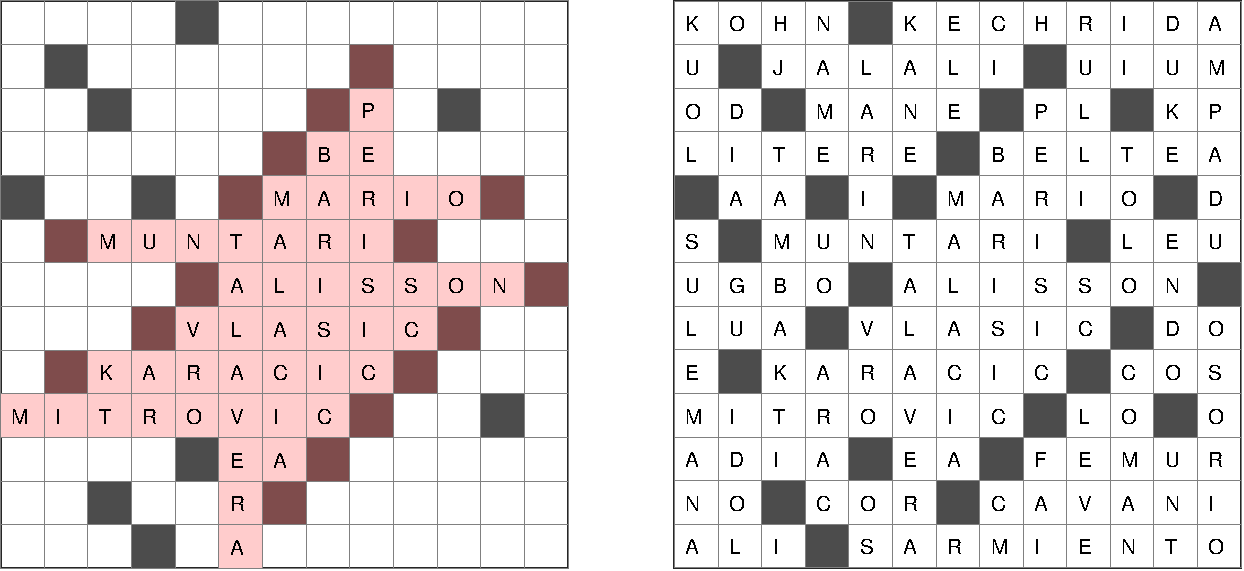
\includegraphics[width=0.6\textwidth]{_empiricalSupport/y-2023/results/_runWombat/mrmeGrids_y2023-60x446-14400x352-14179462-paper.pdf}

\caption{Left: the highest-score synthesized grids for years 2013 (top row), 2021 (middle row) and 2023 (bottom row). The red-tinted black cells and letters come from the seed. Non-tinted black cells are added by the evolution of the seed. Right: {\sc Wombat} solutions for the synthesized grids. The solution scores are 182 (year 2013), 190 (year 2021) and 186 (year 2023).}
\label{fig:results}
\end{figure*}

We applied the approach presented above to synthesize grids for three years of the competition: 2013, 2021 and 2023. Each year uses its own thematic dictionary. Note that competition results and human-designed grids for year 2023 are not yet announced.

For each of the three years we generated and expanded cores (lines~\ref{algl:generateCores} and \ref{algl:expandCores} in Algorithm~\ref{algo:core-exp}), generated seeds (line~\ref{algl:generateSeeds}) that were then ranked (line~\ref{algl:rankSeeds}). Top-ranked seeds were then evolved (line~\ref{algl:evolveSeeds}). The number of seeds ranked and top-ranked seeds evolved are listed in Table~\ref{tab:rankingEvolving}.


The ranking and evolution steps were repeated four times for the same seed set for each year. Each run used a different random-number generator initialization. As per Section~\ref{sec:evolution}, each ranking + evolution run took about two days on a $32$-core CPU. We used four $32$-core CPU nodes on a grid and thus were able to execute all four runs in parallel. The highest score grids synthesized for each year are shown in Figure~\ref{fig:results}. 

The human competition publishes the top 12 entries every year.
In 2013, scores in the top 12 list ranged from 184 (first place), to 181 (second place), and so on down to 175 on the twelfth place.
Our score for that year is 182.
In 2021, human scores in the top-12 list range from 195 down to 187, whereas our score is 190.
2023 human results are not announced yet.

\vb{Adi: please comment on how good those results are and where this places us among the competition grids for those years.}

\vb{Adi: please also remind the reader how little initial information the process needed to derive those grids (so that the reader does not think we took published human grids and did something to them}

